\documentclass{article}
\usepackage{amsmath,mathtools}
\usepackage{graphicx}
\bibliographystyle{IEEEtran}
\usepackage{caption}
\usepackage{subcaption}

\usepackage{boxedminipage}
%\usepackage{geometry}
\usepackage[colorlinks=true]{hyperref}
\title{Notes}
\begin{document}
\maketitle
\section{Computation of Weights map}

\begin{enumerate}
\item The method currently used in paper (Method-1) is:

\begin{equation}
  \boldsymbol{W_v}(x,y,z) = \frac{1}{1+k(\min_{j}|X^j(x,y,z) - P^j(x,y,z)|)}.
  \label{eq:weightsEq}
\end{equation}

\item 
  Let $X_i$ be pilot reconstruction by $i^{th}$ method.\\
  Let $P_i$ be projection of $X_i$ on eigen-space of templates reconstructed using $i^{th}$ method.\\
  If $|X_i-P_i|$ is high, it denotes a new region (region of interest).\\
  If $|X_i-P_i|$ is low, it denotes an old region (where test=templates).
\item \textbf{Illustration of the problem in current method:}\\
  Let there be $6$ different pilot techniques.\\
  Let image intensities be in the range $(0,255)$.\\
  \textbf{Case 1:} Let $|X_i-P_i|$ for each of these methods be $180, 149, 230, 144, 160, 150$. Here, all methods indicate the presence of a new region.
  As per, Eq.~\ref{eq:weightsEq}, $min(.)$ gives $144$. Ideally, we want to select $230$ since this denotes the presence of new region with highest confidence.\\
  \textbf{Case 2: }Now let $|X_i-P_i|$ for each of the methods be $150, 20, 5, 101, 56, 17$. Here most methods (those giving $20, 5, 17, 56$ indicate no presence of new region. However, there are (two false positives) two methods (those giving $101, 150$) that denote the presence of new region.\\
  As per Eq.~\ref{eq:weightsEq}, $min(.)$ gives $5$ which is correct.\\

\item \textbf{Method to correct inaccuracy in Case 1:}\\
  Cluster the $|X_i-P_i|$ into two clusters $C_1$ and $C_2$, with $C_1$ indicating the cluster with lower mean-intensity.\\
  If $C_1$ has more elements than $C_2$, then most methods are indicating that there are no new structures. Here, pick the $min(.)$ of $C_1$ to select the value that indicates no new structures with maximum confidence (i.e., least difference between $X$ and $P$) .\\
  If $C_1$ has fewer elements than $C_2$, then most methods indicate presence of new structure. Here, choose $max(.)$  of $C_2$ to select the value that indicates new structure with maximum confidence (i.e., largest difference between $X$ and $P$).\\

\item However, inorder to create two clusters, we need a threshold.   
\item \textbf{Results using the new method}:\\
  Let threshold be 100.\\
  \textbf{Case 1:} Two clusters are $\{\emptyset\}$ and $\{180, 149, 230, 144, 160, 150\}$. Here, $max(.)$ on $C_2$ will give 230, as expected.\\
  \textbf{Case 2:} Two clusters are $\{20, 5, 56, 17\}$ and $\{150, 101\}$. Here, $C_1$ has more elements. There, we take a $min(.)$ and get $5$ ( same as our current method).

\item {\textbf{Method-2:}}\\
  
 
\[
     \boldsymbol{W_v}(x,y,z)= 
\begin{dcases}
    \frac{1}{(1+k(\min_{j\in C_1}|X^j(x,y,z) - P^j(x,y,z)|))},& \text{if } |C_1|>|C_2|\\
    \frac{1}{(1+k(\max_{j\in C_2}|X^j(x,y,z) - P^j(x,y,z)|))},              & \text{otherwise}
\end{dcases}
\]

\item \textbf{Method-3:}\\
  \begin{equation}
    \boldsymbol{W_v}(x,y,z) = \frac{1}{1+k(\textrm{median}_{j}|X^j(x,y,z) - P^j(x,y,z)|)}.
    \label{eq:weightsEqMethod3}
  \end{equation}

  No threshold is needed here. Accuracy of this method may be better than method-1 and worse than method-2.\\

  \textbf{Case 1:} Ordered set = $\{144, 149, 150, 160, 180, 230\}$. Median $= 155$. (Method-1 gives 144. Method-2 gives 230;  Ideal value is 230.)\\
  \textbf{Case 2:} Ordered set = $\{5, 20, 17, 56, 101, 150\}$. Median $= 36.5$ (Method-1 gives 5, Method-2 gives 5. Ideal value is 5.)
  
\end{enumerate}

%-------------------------------------------------------------------------------
\section{Computing sufficient level of subsampling}

\subsection{2D}

\begin{enumerate}
\item Let $N$ be the total number of views. 
\begin{figure}[!h]
\centering
	\includegraphics[width=0.5\textwidth]{../images/notes_1.png}
        \caption{2D image of size [D,D]. Ray at $45^\circ$}
 \label{fig:prior_overview}
\end{figure}


\begin{figure}[!h]
\centering
	\includegraphics[width=0.5\textwidth]{../images/notes_2.png}
        \caption{In order to find $N$, consider the image to be fit within a circle of radius $r = \frac{D\sqrt2}{2}$. }
 \label{fig:prior_overview}
\end{figure}


\begin{figure}[!h]
\centering
	\includegraphics[width=0.5\textwidth]{../images/notes_3.png}
        \caption{Consider the same circle, now with ray from all views. The innermost pixels will have maximum number of rays passing through them. The outermost pixels will have minimum number of rays passing through them.}
 \label{fig:prior_overview}
\end{figure}

\begin{figure}[h]
\centering
	\includegraphics[width=0.5\textwidth]{../images/notes_4.png}
        \caption{We must ensure that there is atleast one ray passing through each outermost pixel.}
 \label{fig:prior_overview}
\end{figure}
\clearpage
\item
  \begin{align}
    N &= \frac{2\pi r}{2}\\
    &= \frac{\pi D}{\sqrt2}
  \end{align}

\item For okra, [310,310] image, N = 688.\\
 For sprouts, [260,260] image, N = 577\\
 For potato, [150, 150] image, N = 333\\
\end{enumerate}

\subsection{3D}
\begin{enumerate}
\item Here, The volume of size $[D, D, D]$ is fit within sphere of radius $\frac{\sqrt3D}{2}$.


  \begin{align}
    N &= \frac{4\pi r^2}{2}\\
    &= \frac{3\pi D^2}{2}
  \end{align}
\end{enumerate}

\end{document}


  \item At any degree, we assume atleast one ray must pass through each pixel in the longest perpendicular path to the ray within the image. For example,  At $45^\circ$ view, atleast one ray must pass through each pixel on the leading diagonal.

   \item (One ray per corner pixel helps us to find the value of the corner pixel directly.)


\item Therefore, let total number of rays be $\sqrt2DN$, where $\sqrt2$ is the number rays per view and $N$ is the total number of view.
